\documentclass{article}
\usepackage{amsmath}
\usepackage{amsthm}
\usepackage{amsfonts}
\usepackage{amssymb}
\usepackage{bbold}
\usepackage{dsfont}
\usepackage{graphicx}
\usepackage{cleveref}
\usepackage{bm}
\usepackage{booktabs}
\usepackage{siunitx}
\usepackage{xcolor}
\usepackage[utf8]{inputenc}
\usepackage[english]{babel}
\newtheorem{definition}{Definition}
\newtheorem{example}{Example}
\newcommand{\exP}[1]{\mathrm{e}^{#1}}
\newcommand{\dif}{\mathrm{d}}
\renewcommand{\vec}[1]{\mathbf{#1}}
\newcommand{\pdagger}{{\phantom{\dagger}}}
\newcommand{\state}[1]{\vert #1\rangle}
\newcommand{\cstate}[1]{\langle #1\vert}
\newcommand{\tr}[1]{\mathrm{tr}\left\{#1\right\}}
\newcommand{\trs}[2]{\, \mathrm{tr}_{#1}\{#2\}}
\newcommand{\expc}[3]{\langle #1\vert #2 \vert #3\rangle}
\usepackage[doi=false,url=false,isbn=false,backend=bibtex,style=nature,natbib=true,sorting=none]{biblatex}
\bibliography{bib.bib}
\usepackage{geometry}
\geometry{
	a4paper,
	total={170mm,257mm},
	left=20mm,
	top=20mm,
}
\begin{document}
	
\title{Fransson's model: Tests of implementation}
\author{Rudolf Smorka}
\maketitle
\section{Model}
The model considered for a chiral, single-stranded molecule, as proposed in Refs.~\cite{fransson2019chirality,fransson2020vibrational,Fransson_2021,fransson2021charge}, reads
\begin{align}
	\hat{H} &= \hat{H}_\mathrm{mol} + \hat{H}_\mathrm{env} + \hat{H}_\mathrm{sys-env}.
\end{align} 
The molecular Hamiltonian consists of a electronic on-site, nearest-neighbor hopping, and next-to-nearest neighbor spin-orbit coupling (SOC), a Peierls electron-phonon coupling and vibrational contribution to SOC, and the harmonic phonon potential energy 
\begin{align}
	\hat{H}_\mathrm{mol} &= \hat{H}_\mathrm{el} + \hat{H}_\mathrm{el-ph} + \hat{H}_\mathrm{ph},\\
	\begin{split}
		\hat{H}_\mathrm{el} &= \sum_{j,\sigma} \varepsilon_{j\sigma}^\pdagger \hat{d}_{j\sigma}^\dagger \hat{d}_{j\sigma}^\pdagger - t_0 \sum_{j\sigma} (\hat{d}_{j\sigma}^\dagger \hat{d}_{j+1,\sigma}^\pdagger + \mathrm{h.c.}) +\\& \lambda_0^\pdagger\sum_{j\sigma\sigma'} (i\hat{d}_{j\sigma}^\dagger (\vec{v}_j^{(+)}\cdot \bm{\sigma})_{\sigma\sigma'}^\pdagger \hat{d}_{j+2,\sigma'}^\pdagger + \mathrm{h.c.}),
	\end{split}\\
	\hat{H}_\mathrm{el-ph} &= - t_1^\pdagger \sum_{j,\sigma}  \hat{d}_{j\sigma}^\dagger \hat{d}_{j+1\sigma}^\pdagger (\hat{a}_{j}^\dagger + \hat{a}_{j}^\pdagger) \\ & + \lambda_1^\pdagger\sum_{j\sigma} (i \hat{d}_{j\sigma}^\dagger (\vec{v}_j^{(+)} \cdot \bm{\sigma})_{\sigma\sigma'}^\pdagger \hat{d}_{j+2\sigma'}^\pdagger +\mathrm{h.c.})(\hat{a}_{j}^\dagger + \hat{a}_{j}^\pdagger),\label{eq:HelPh}\\
	\hat{H}_\mathrm{ph} &= \sum_{j} \omega_{j}^\pdagger \hat{a}_{j}^\dagger \hat{a}_{j}^\pdagger.
	 \label{eq:Hamiltonian_el_Fransson} 
\end{align}
This molecule is coupled to an environment of spin-full, noninteracting electrons
\begin{equation}
	H_\mathrm{env} = \sum_{\ell k\sigma} \varepsilon_{\ell k\sigma}^\pdagger c_{\ell k\sigma}^\dagger c_{\ell k\sigma}^\pdagger \label{eq:LeadHamiltonian}
\end{equation}
and the system-environment coupling is linear in the molecular and environmental operators (only at the first and last site of the molecule)
\begin{align}
	H_\mathrm{sys-env} &= \sum_{\sigma\sigma'}(\nu_{L\sigma\sigma'}^\pdagger c_{N_L\sigma}^\dagger d_{1\sigma'}^\pdagger + \nu_{R\sigma\sigma'}^\pdagger c_{1_R\sigma}^\dagger d_{\mathbb{M}\sigma'}^\pdagger + \mathrm{h.c.}). \label{eq:LeadSysHamiltonian}
\end{align} 
\section{Methods}
In the following, we compare the dynamics in the model defined above using a variety of methods. 
\begin{itemize}
	\item Exact diagonalization (ED): Valid for isolated molecule, phonons treated quantum-mechanically.
	\item Time-dependent variational principle based on a matrix-product state Ansatz (TDVP): Valid for isolated molecule, phonons treated quantum-mechanically.
	\item Hierarchical equations of motion in matrix product state representation (TT-HEOM): Valid for both isolated molecule and molecule coupled to leads, phonons treated quantum-mechanically.
	\item Hierarchical equations of motion in combination with Ehrenfest dynamics (MF-HEOM): Valid for purely electronic dynamics in both isolated molecule and molecule coupled to leads. Phonons approximated to be classical.
\end{itemize}
\newpage
\section{Comparison of Dynamics in Isolated Molecule}
\subsection{Static Molecule}
\subsubsection{On-site and Hopping}
Parameters: $L=3$, $t_0 = 1$, $\varepsilon_\uparrow = 1= -\varepsilon_\downarrow$. 
\begin{figure}[!h]
	\centering
	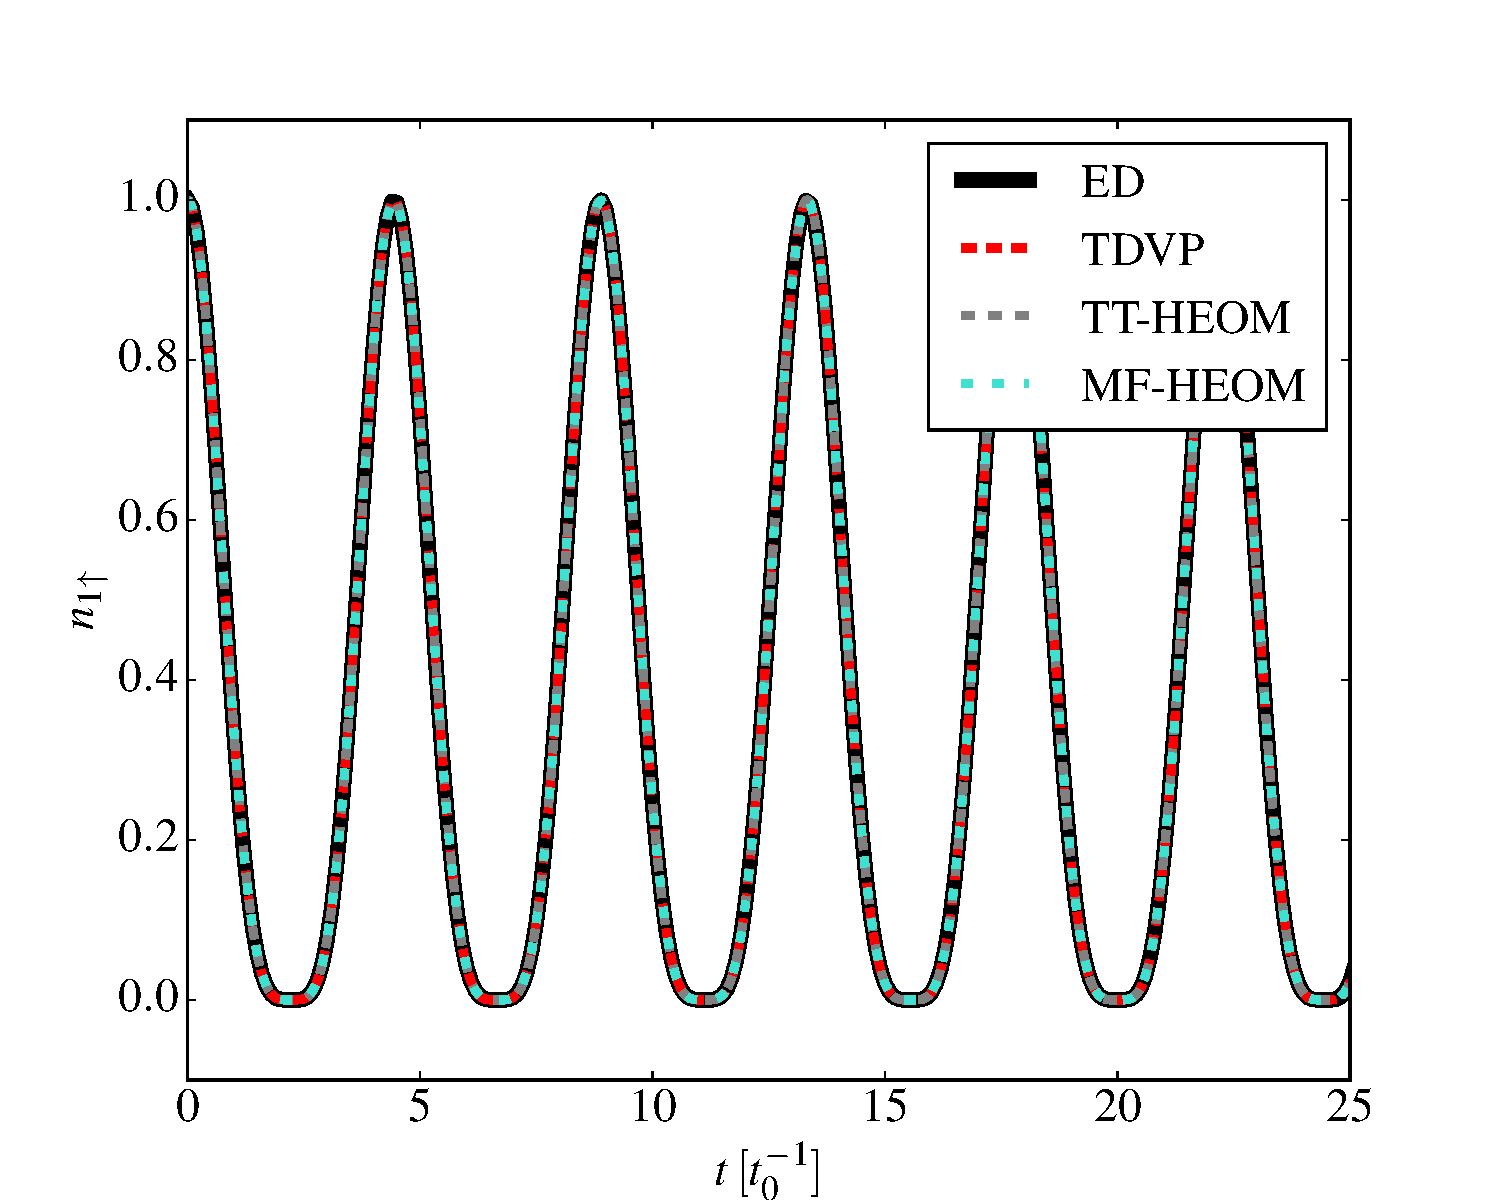
\includegraphics[width=0.74\textwidth]{figs/Comparison_TTHEOM_MFHEOM_TDVP_ED_hop+onsite.pdf}
\end{figure}
\subsubsection{On-site, Hopping, and SOC}
Parameters: $L=3$, $t_0 = 1$, $\varepsilon_\uparrow = 1= -\varepsilon_\downarrow$, $\lambda = 0.8$. 
\begin{figure}[!h]
	\centering
	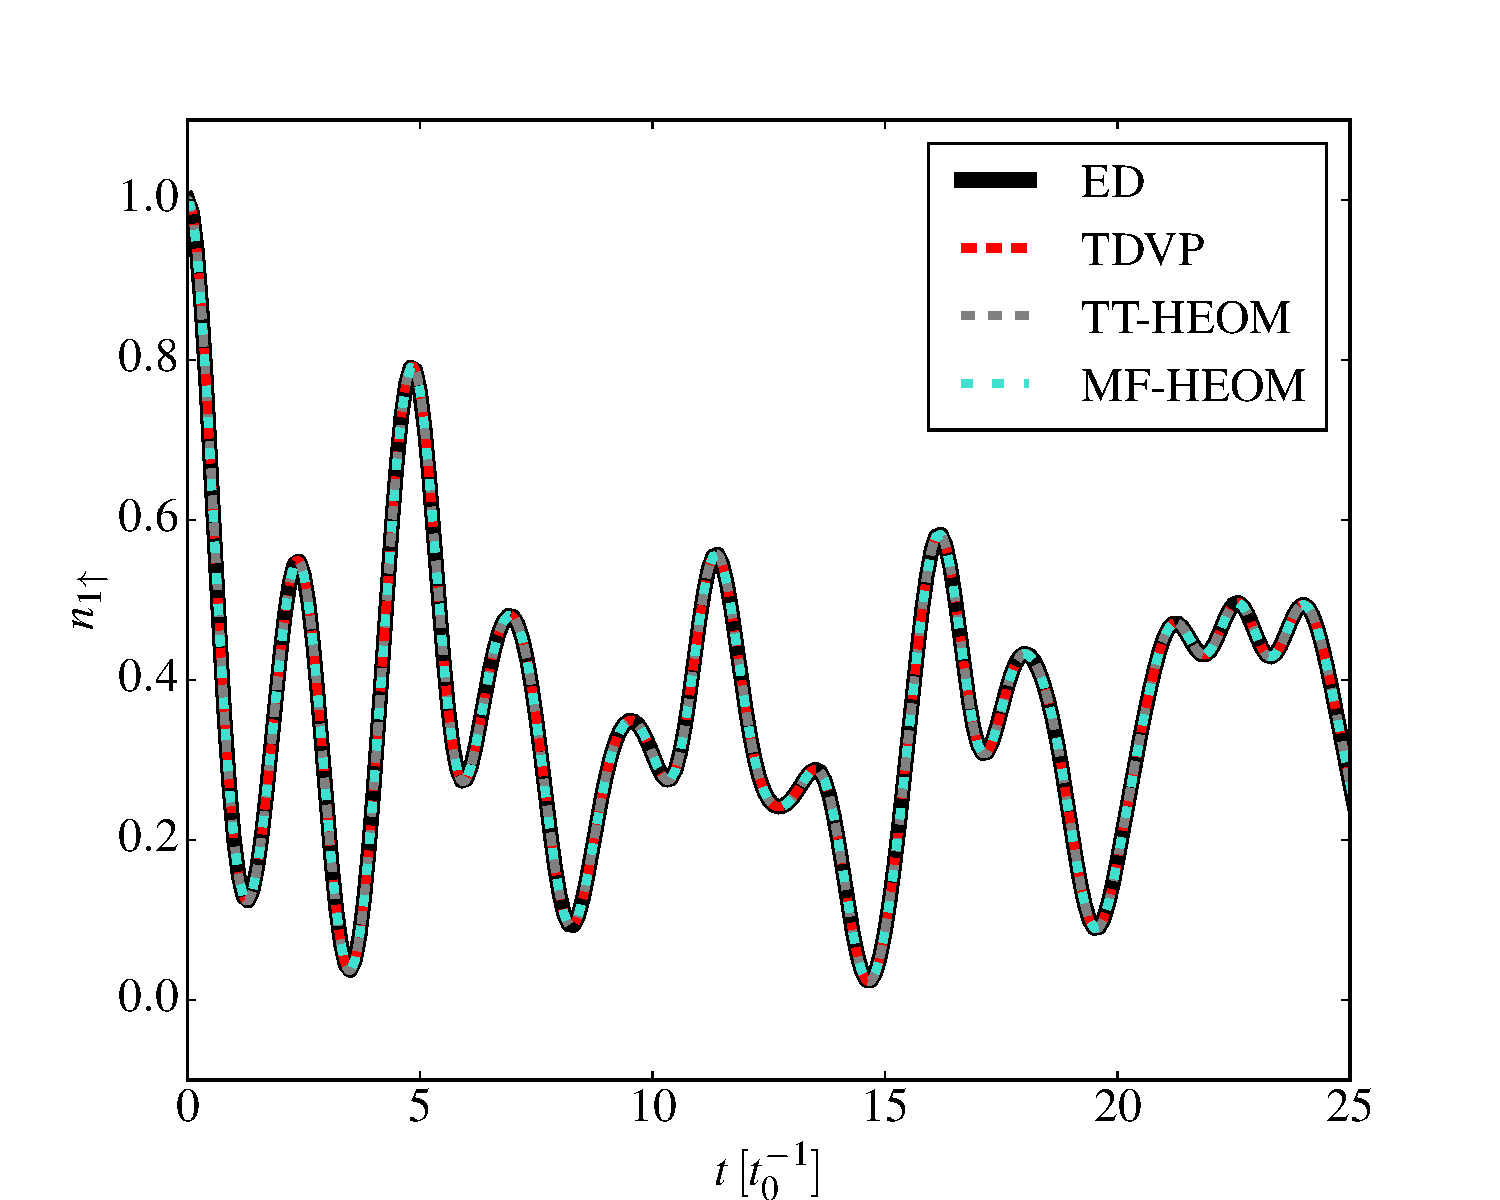
\includegraphics[width=0.74\textwidth]{figs/Comparison_TTHEOM_MFHEOM_TDVP_ED_hop+onsite+soc.pdf}
\end{figure}
\subsection{Vibrating molecule}
\subsubsection{Hopping and Peierls distortion}
Parameters: $L=3$, $t_0 = 1$, $t_1 = 0.1t_0$. 

\begin{figure}[!h]
	\centering
	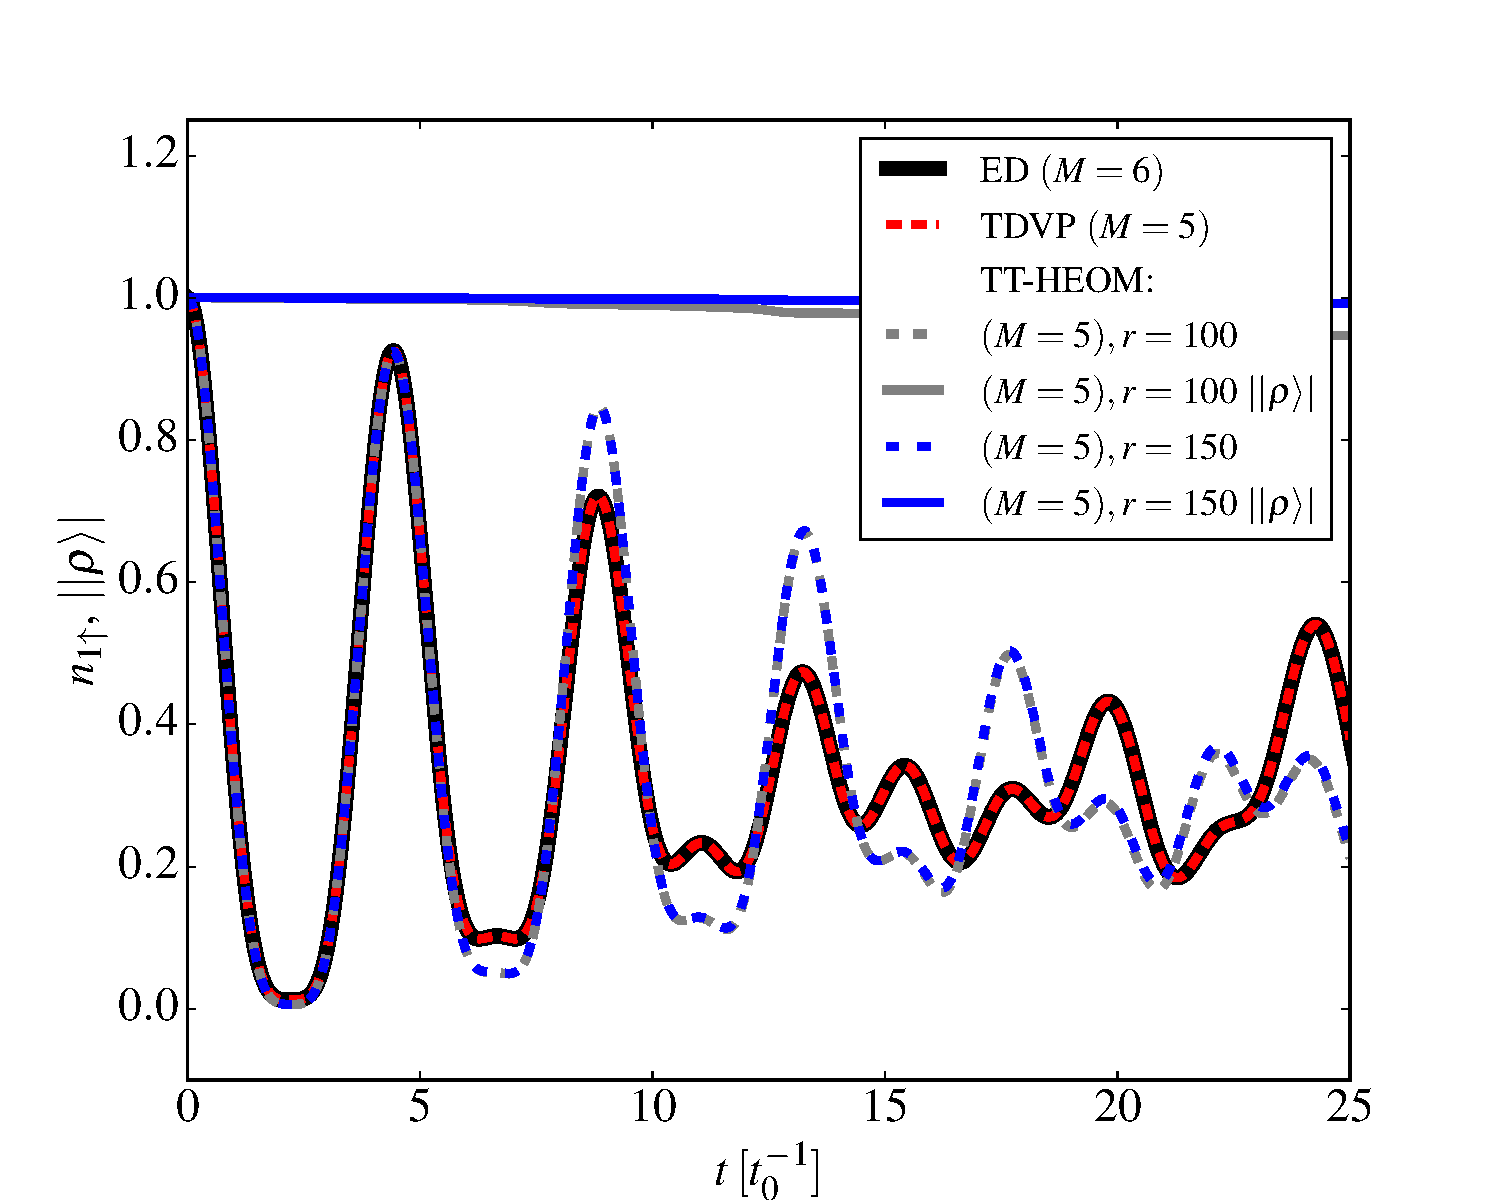
\includegraphics[width=0.9\textwidth]{figs/Comparison_TTHEOM_TDVP_ED_hop+onsite+tph.pdf}
\end{figure}
\subsubsection{Hopping, SOC, and Peierls distortion}
Parameters: $L=3$, $t_0 = 1$, $\lambda_0 = t_0/40$, $t_1 = 0.1t_0$. 

\subsubsection{Hopping, SOC, Peierls distortion, and Peierls-SOC}
Parameters: $L=3$, $t_0 = 1$, $\lambda_0 = t_0/40$, $t_1 = 0.1t_0$, $\lambda_1 = 0.1\lambda_0$. 

\section{Comparison of Dynamics in Open Molecule}
\subsection{No vibrations}
\subsubsection{Hopping}
Parameters: $L=3$, $t_0 = 1$, $\Gamma = 0.5t_0$, $V=1$, $\beta = 1/0.026$. 
\subsubsection{Hopping and SOC}
\subsection{With vibrations}
\subsubsection{Hopping, SOC and Peierls distortion}
\subsubsection{Hopping, SOC, Peierls distortion and Peierls SOC}



\printbibliography
\end{document}




